\section{Zielsetzung}
In diesem Versuch wird zunächst die Zeitkonstante eines RC-Kreises bestimmt.
Anschließend wird die Amplitude der Kondensatorspannung in Abhängigkeit der Frequenz und
die Phasenverschiebung von Kondensator- und Generatorspannung ebenfalls in Abhängigkeit der
Frequenz gemessen. Zum Schluss wird gezeigt, dass der RC-Kreis Spannungen
integrieren kann.

\section{Theorie}
\subsection{RC-Kreis und Relaxationsverhalten}
Ein System zeigt ein Relaxationsverhalten, wenn es aus seinem Ausgangszustand
ausgelenkt wurde und nicht-oszillatorisch in diesen zurückkerhrt. Dabei ist die
Änderungsgeschwindigkeit der Größe $A$ zum Zeitpunkt $t$ meist proportional zur
Abweichung von A zum Endzustand A(\infty)
\begin{equation}
  \frac{dA}{dt} = c[A(t)-A(\infty)].
  \label{eqn:diff1}
\end{equation}
Duch Integration diese Gleichung von 0 bis $t$ folgt
\begin{equation}
  A(t)=A(\infty)+[A(0)-A(\infty)] \cdot \exp{(ct)}
\end{equation}
womit A zum Zeitpunkt $t$ berechnet weden kann.
Dabei muss c$\:$<$\:$0 gelten, damit A beschränkt bleibt. \\

\noindent Ein Beipiel für Relaxationsvorgänge ist das Auf- und Endladen eines Kondensators
über einen Widerstand.
\begin{figure}[H]
  \centering
  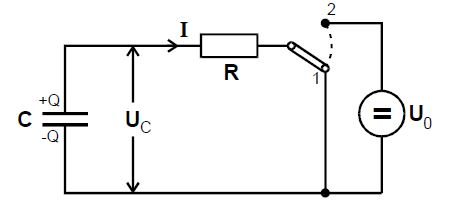
\includegraphics[height=5cm]{RC.JPG}
  \caption{Entladung (Stellung 1) und Aufladung (Stellung 2) eines RC-Kreises.}
  \cite{skript}
  \label{fig:RC}
  \end{figure}

\noindent \textbf{Entladung eines Kondensators}\\
\label{sec:Entladung}
Für die Spannung $U_{C}$ am Kondensator mit der Kapazizät C und der Ladung Q gilt:
\begin{equation}
  U_{C} = \frac{Q}{C}.
  \label{Spannung}
\end{equation}
Mit Hilfe des ohmschen Gesetzes $U=R\cdot I$ und der Beziehung $\dot{Q}=I$
folgt aus \eqref{eqn:Spannung} eine Differentialgleichung für die Ladung des
Kondensators.
\begin{equation}
  \frac{dQ}{dt}=- \frac{1}{RC}\; Q(t)
  \label{eqn:diff2}
\end{equation}
Diese Differentialgleichung hat die gleiche Gestallt wie Gleichung \eqref{eqn:diff1}.
Mit der Annahme, dass der Kondensator nach $t \to \infty$ entladen ist, folgt
nach Integration
\begin{equation}
  Q(t)=Q(0)\exp{\left(\frac{-t}{RC}\right)}.
  \label{eqn:entladung}
\end{equation}

\noindent \textbf{Aufladen eines Kondensators} \\
Ähnlich wie in Abschnitt \ref{sec:Theorie} kann eine Gleichung für den
Aufladevorgang des Kondensators hergeleitet werden. Hier gelten die
Randbedingungen $Q(0)=0$ und $Q(\infty)=CU_{0}$. Somt ergibt sich
für den Aufladevorgang mit einer äußeren Spannungsquelle der Spannung $U_{0}$
die Gleichung
\begin{equation}
  Q(t)=CU_{0}\left(1-\exp{\left(\frac{-t}{RC}\right)}\right).
  \label{aufladen}
\end{equation}
Dabei wird der Ausdruck RC als Zeitkonstante des Relaxationsvorganges bezeichnet,
er ist ein Maß für die Geschwindigkeit, mit der das System seinem Endzusand entgegenstrebt.\\
\\
\subsection{Relaxationsvorgänge mit periodischer Auslenkung}
Wenn ein System von außen periodisch aus seiner Gleichgewichtslage ausgelenkt wird
treten ebenfalls Relaxationsvorgänge auf. In dem Beipiel des RC-Kreises wird
das System mit einer Wechselspannung ausgelenkt, wie in Abbildung \ref{fig:RCsin}
zu sehen.
\begin{figure}[H]
  \centering
  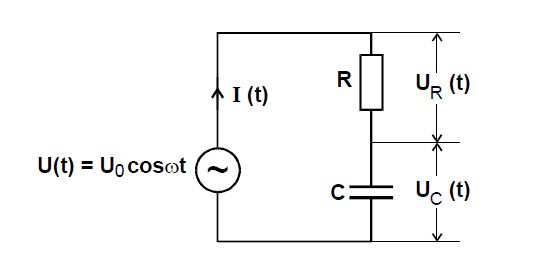
\includegraphics[height=5cm]{RCsin.JPG}
  \caption{Periodische Anregung eines RC-Kreises.}
  \cite{skript}
  \label{fig:RCsin}
\end{figure}
An die Schaltung wird eine äußere Wechselspannung
\begin{equation}
  U(t)=U_{0}\cos(\omega t)
\end{equation}
mit der Kreisfrequenz $\omega$ angelegt. Gilt ür diese $\omega<<1/RC$, so ist
die Spannung $U_{C}$ am Kondensator nachezu der angelegten Spannung $U(t)$.
Mit steigender Frequenz sinkt die Amplitude von $U_{C}$ und es bildet sich eine
Phasenverschiebung $\phi$ aus, da Auf- und Entladung des Kondensators immer weiter
hinter der angelegten Spannung zurückbleiben.
Für diesen Problem wird folgender Ansatz gemacht:
\begin{equation}
  U_{C}(t)=A(\omega)\cos(\omega t + \phi(\omega)).
\end{equation}
Mit dem zweiten Kirchhoffschen Gesetz und weitern Umformungen folgt:
\begin{equation}
  \phi(\omega)= \arctan(-\omega RC)
  \label{eqn:phi}
\end{equation}
für die Frquenzabhängigkeit der Phasenverschiebung.
An dieser Formel wird deutlich, dass die Phasenverschiebung für sehr kleine
$\omega$ gegen Null geht und sich für große $\omega$ dem Wert $\frac{\pi}{2}$
annähert.
Aus weiteren Rechnungen folgt für die Frequenzabhängigkeit der Amplitude der
Kondensatorspannung
\begin{equation}
  A(\omega)=\frac{U_{0}}{\sqrt{1+(\omega RC)^2}}.
  \label{eqn:amplitude}
\end{equation}
Daus ergibt sich, dass $A(\omega)$ für $\omega \to 0$ gegen $U_{0}$ geht und
für $\omega \to \infty$ gegen Null geht. Für $\omega = 1/RC$ ergibt sich für $A(\omega)$
$U_{0}/\sqrt{2}$.
Da von dieser RC-Schaltung niedrige Frequenzen durchgelassen werden und
hohe Frequenzen nicht, wird diese Schaltung auch als Tiefpass bezeichnet.
\subsection{RC-Kreis als Integrator}
Gilt für die äußere angelegte Frequenz $\omega >> 1/RC$, so kann gezeigt weden, dass
ein RC-Kreis wie in Abbildung \ref{fig:RCsin} eine periodische Spannung integrieren kann.
Unter diesen Vorraussetzungen gilt:
\begin{equation}
  U_{C}(t)=\frac{1}{RC}\int_{0}^{t} U(t')dt'.
  \label{eqn:integral}
\end{equation}

\label{sec:Theorie}

%\cite{sample}
